\documentclass[1p]{elsarticle_modified}
%\bibliographystyle{elsarticle-num}

%\usepackage[colorlinks]{hyperref}
%\usepackage{abbrmath_seonhwa} %\Abb, \Ascr, \Acal ,\Abf, \Afrak
\usepackage{amsfonts}
\usepackage{amssymb}
\usepackage{amsmath}
\usepackage{amsthm}
\usepackage{scalefnt}
\usepackage{amsbsy}
\usepackage{kotex}
\usepackage{caption}
\usepackage{subfig}
\usepackage{color}
\usepackage{graphicx}
\usepackage{xcolor} %% white, black, red, green, blue, cyan, magenta, yellow
\usepackage{float}
\usepackage{setspace}
\usepackage{hyperref}

\usepackage{tikz}
\usetikzlibrary{arrows}

\usepackage{multirow}
\usepackage{array} % fixed length table
\usepackage{hhline}

%%%%%%%%%%%%%%%%%%%%%
\makeatletter
\renewcommand*\env@matrix[1][\arraystretch]{%
	\edef\arraystretch{#1}%
	\hskip -\arraycolsep
	\let\@ifnextchar\new@ifnextchar
	\array{*\c@MaxMatrixCols c}}
\makeatother %https://tex.stackexchange.com/questions/14071/how-can-i-increase-the-line-spacing-in-a-matrix
%%%%%%%%%%%%%%%

\usepackage[normalem]{ulem}

\newcommand{\msout}[1]{\ifmmode\text{\sout{\ensuremath{#1}}}\else\sout{#1}\fi}
%SOURCE: \msout is \stkout macro in https://tex.stackexchange.com/questions/20609/strikeout-in-math-mode

\newcommand{\cancel}[1]{
	\ifmmode
	{\color{red}\msout{#1}}
	\else
	{\color{red}\sout{#1}}
	\fi
}

\newcommand{\add}[1]{
	{\color{blue}\uwave{#1}}
}

\newcommand{\replace}[2]{
	\ifmmode
	{\color{red}\msout{#1}}{\color{blue}\uwave{#2}}
	\else
	{\color{red}\sout{#1}}{\color{blue}\uwave{#2}}
	\fi
}

\newcommand{\Sol}{\mathcal{S}} %segment
\newcommand{\D}{D} %diagram
\newcommand{\A}{\mathcal{A}} %arc


%%%%%%%%%%%%%%%%%%%%%%%%%%%%%5 test

\def\sl{\operatorname{\textup{SL}}(2,\Cbb)}
\def\psl{\operatorname{\textup{PSL}}(2,\Cbb)}
\def\quan{\mkern 1mu \triangleright \mkern 1mu}

\theoremstyle{definition}
\newtheorem{thm}{Theorem}[section]
\newtheorem{prop}[thm]{Proposition}
\newtheorem{lem}[thm]{Lemma}
\newtheorem{ques}[thm]{Question}
\newtheorem{cor}[thm]{Corollary}
\newtheorem{defn}[thm]{Definition}
\newtheorem{exam}[thm]{Example}
\newtheorem{rmk}[thm]{Remark}
\newtheorem{alg}[thm]{Algorithm}

\newcommand{\I}{\sqrt{-1}}
\begin{document}

%\begin{frontmatter}
%
%\title{Boundary parabolic representations of knots up to 8 crossings}
%
%%% Group authors per affiliation:
%\author{Yunhi Cho} 
%\address{Department of Mathematics, University of Seoul, Seoul, Korea}
%\ead{yhcho@uos.ac.kr}
%
%
%\author{Seonhwa Kim} %\fnref{s_kim}}
%\address{Center for Geometry and Physics, Institute for Basic Science, Pohang, 37673, Korea}
%\ead{ryeona17@ibs.re.kr}
%
%\author{Hyuk Kim}
%\address{Department of Mathematical Sciences, Seoul National University, Seoul 08826, Korea}
%\ead{hyukkim@snu.ac.kr}
%
%\author{Seokbeom Yoon}
%\address{Department of Mathematical Sciences, Seoul National University, Seoul, 08826,  Korea}
%\ead{sbyoon15@snu.ac.kr}
%
%\begin{abstract}
%We find all boundary parabolic representation of knots up to 8 crossings.
%
%\end{abstract}
%\begin{keyword}
%    \MSC[2010] 57M25 
%\end{keyword}
%
%\end{frontmatter}

%\linenumbers
%\tableofcontents
%
\newcommand\colored[1]{\textcolor{white}{\rule[-0.35ex]{0.8em}{1.4ex}}\kern-0.8em\color{red} #1}%
%\newcommand\colored[1]{\textcolor{white}{ #1}\kern-2.17ex	\textcolor{white}{ #1}\kern-1.81ex	\textcolor{white}{ #1}\kern-2.15ex\color{red}#1	}

{\Large $\underline{12a_{1160}~(K12a_{1160})}$}

\setlength{\tabcolsep}{10pt}
\renewcommand{\arraystretch}{1.6}
\vspace{1cm}\begin{tabular}{m{100pt}>{\centering\arraybackslash}m{274pt}}
\multirow{5}{120pt}{
	\centering
	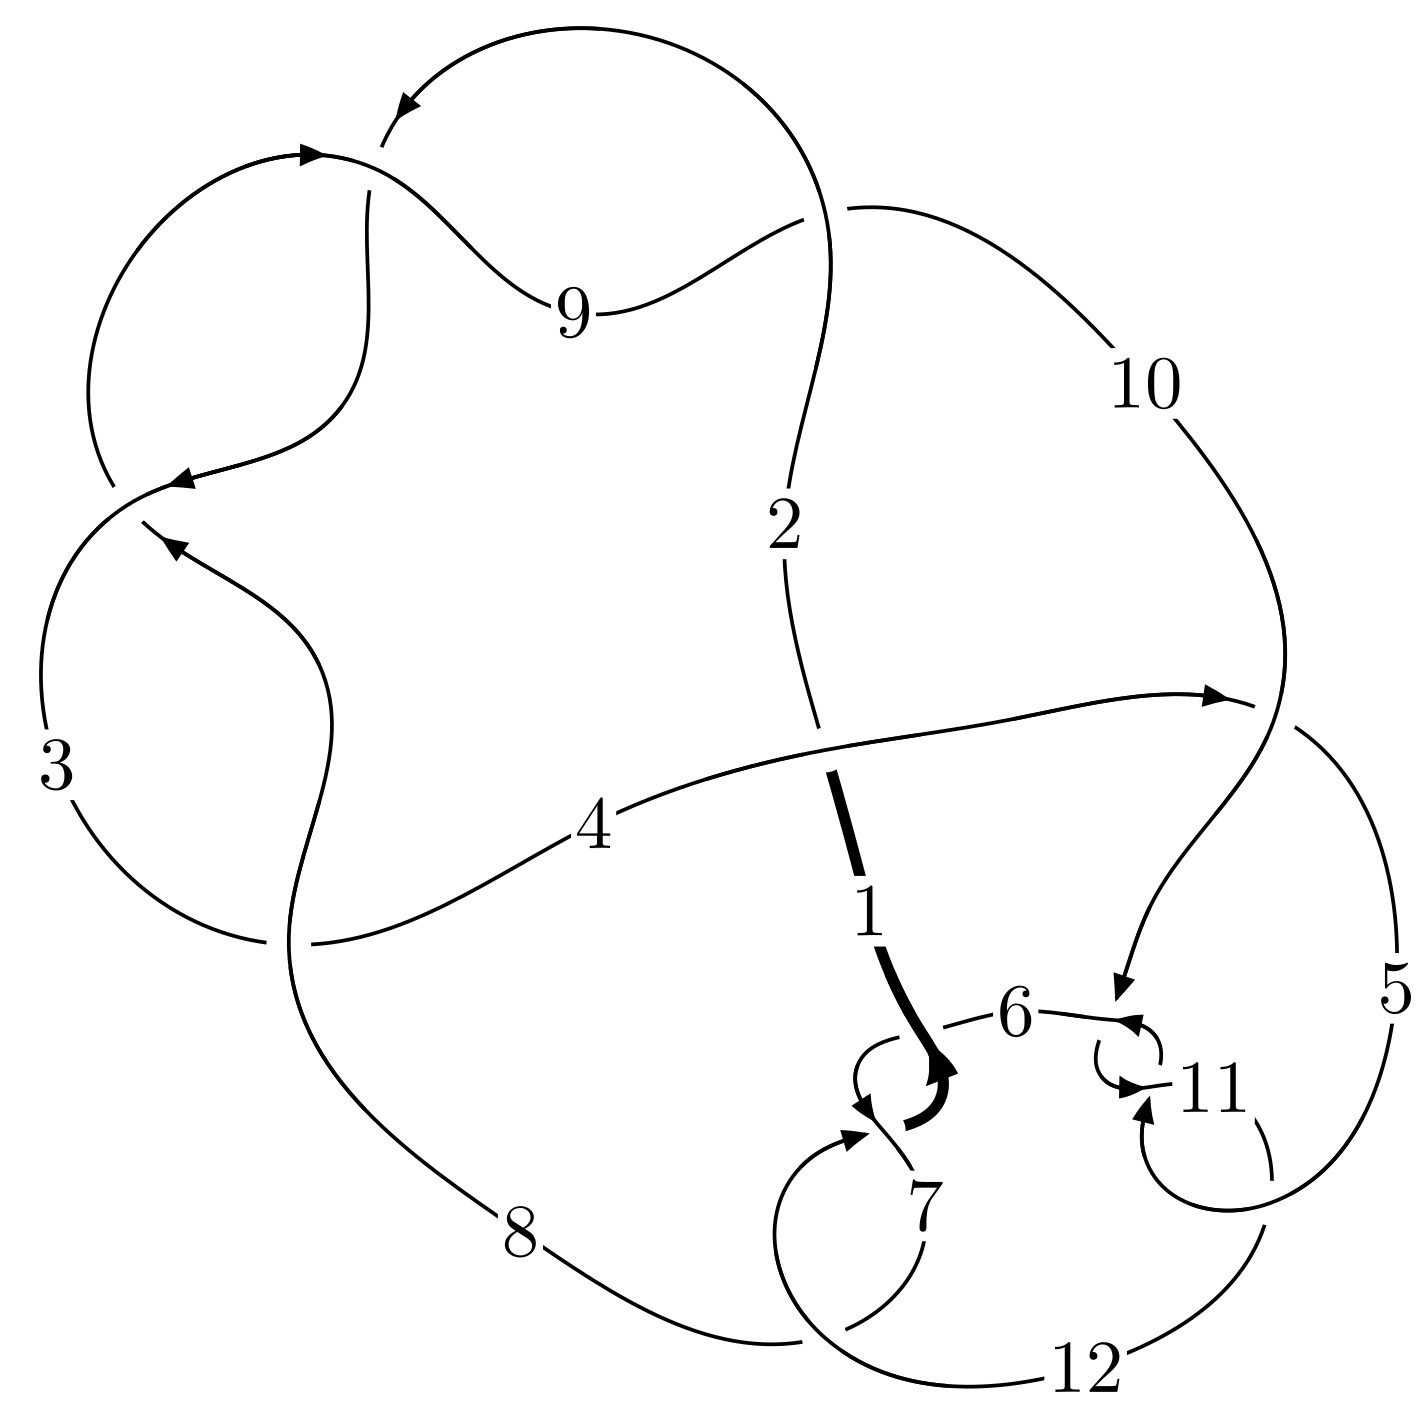
\includegraphics[width=112pt]{../../../GIT/diagram.site/Diagrams/png/1961_12a_1160.png}\\
\ \ \ A knot diagram\footnotemark}&
\allowdisplaybreaks
\textbf{Linearized knot diagam} \\
\cline{2-2}
 &
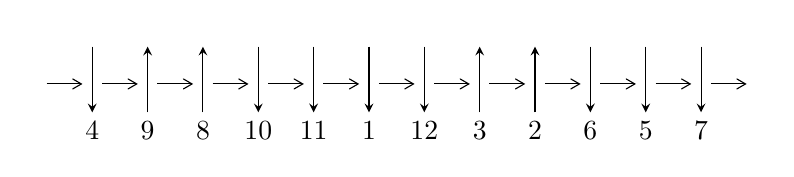
\begin{tikzpicture}[x=20pt, y=17pt]
	% nodes
	\node (C0) at (0, 0) {};
	\node (C1) at (1, 0) {};
	\node (C1U) at (1, +1) {};
	\node (C1D) at (1, -1) {4};

	\node (C2) at (2, 0) {};
	\node (C2U) at (2, +1) {};
	\node (C2D) at (2, -1) {9};

	\node (C3) at (3, 0) {};
	\node (C3U) at (3, +1) {};
	\node (C3D) at (3, -1) {8};

	\node (C4) at (4, 0) {};
	\node (C4U) at (4, +1) {};
	\node (C4D) at (4, -1) {10};

	\node (C5) at (5, 0) {};
	\node (C5U) at (5, +1) {};
	\node (C5D) at (5, -1) {11};

	\node (C6) at (6, 0) {};
	\node (C6U) at (6, +1) {};
	\node (C6D) at (6, -1) {1};

	\node (C7) at (7, 0) {};
	\node (C7U) at (7, +1) {};
	\node (C7D) at (7, -1) {12};

	\node (C8) at (8, 0) {};
	\node (C8U) at (8, +1) {};
	\node (C8D) at (8, -1) {3};

	\node (C9) at (9, 0) {};
	\node (C9U) at (9, +1) {};
	\node (C9D) at (9, -1) {2};

	\node (C10) at (10, 0) {};
	\node (C10U) at (10, +1) {};
	\node (C10D) at (10, -1) {6};

	\node (C11) at (11, 0) {};
	\node (C11U) at (11, +1) {};
	\node (C11D) at (11, -1) {5};

	\node (C12) at (12, 0) {};
	\node (C12U) at (12, +1) {};
	\node (C12D) at (12, -1) {7};
	\node (C13) at (13, 0) {};

	% arrows
	\draw[->,>={angle 60}]
	(C0) edge (C1) (C1) edge (C2) (C2) edge (C3) (C3) edge (C4) (C4) edge (C5) (C5) edge (C6) (C6) edge (C7) (C7) edge (C8) (C8) edge (C9) (C9) edge (C10) (C10) edge (C11) (C11) edge (C12) (C12) edge (C13) ;	\draw[->,>=stealth]
	(C1U) edge (C1D) (C2D) edge (C2U) (C3D) edge (C3U) (C4U) edge (C4D) (C5U) edge (C5D) (C6U) edge (C6D) (C7U) edge (C7D) (C8D) edge (C8U) (C9D) edge (C9U) (C10U) edge (C10D) (C11U) edge (C11D) (C12U) edge (C12D) ;
	\end{tikzpicture} \\
\hhline{~~} \\& 
\textbf{Solving Sequence} \\ \cline{2-2} 
 &
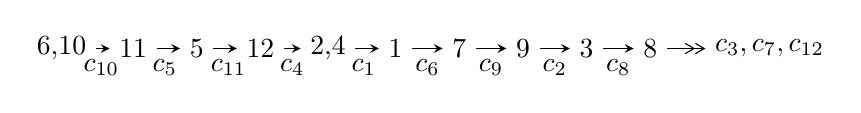
\begin{tikzpicture}[x=23pt, y=7pt]
	% node
	\node (A0) at (-1/8, 0) {6,10};
	\node (A1) at (1, 0) {11};
	\node (A2) at (2, 0) {5};
	\node (A3) at (3, 0) {12};
	\node (A4) at (65/16, 0) {2,4};
	\node (A5) at (41/8, 0) {1};
	\node (A6) at (49/8, 0) {7};
	\node (A7) at (57/8, 0) {9};
	\node (A8) at (65/8, 0) {3};
	\node (A9) at (73/8, 0) {8};
	\node (C1) at (1/2, -1) {$c_{10}$};
	\node (C2) at (3/2, -1) {$c_{5}$};
	\node (C3) at (5/2, -1) {$c_{11}$};
	\node (C4) at (7/2, -1) {$c_{4}$};
	\node (C5) at (37/8, -1) {$c_{1}$};
	\node (C6) at (45/8, -1) {$c_{6}$};
	\node (C7) at (53/8, -1) {$c_{9}$};
	\node (C8) at (61/8, -1) {$c_{2}$};
	\node (C9) at (69/8, -1) {$c_{8}$};
	\node (A10) at (11, 0) {$c_{3},c_{7},c_{12}$};

	% edge
	\draw[->,>=stealth]	
	(A0) edge (A1) (A1) edge (A2) (A2) edge (A3) (A3) edge (A4) (A4) edge (A5) (A5) edge (A6) (A6) edge (A7) (A7) edge (A8) (A8) edge (A9) ;
	\draw[->>,>={angle 60}]	
	(A9) edge (A10);
\end{tikzpicture} \\ 

\end{tabular} \\

\footnotetext{
The image of knot diagram is generated by the software ``\textbf{Draw programme}" developed by Andrew Bartholomew(\url{http://www.layer8.co.uk/maths/draw/index.htm\#Running-draw}), where we modified some parts for our purpose(\url{https://github.com/CATsTAILs/LinksPainter}).
}\phantom \\ \newline 
\centering \textbf{Ideals for irreducible components\footnotemark of $X_{\text{par}}$} 
 
\begin{align*}
I^u_{1}&=\langle 
u^{22}- u^{21}+\cdots+4 b-1,\;u^{22}- u^{21}+\cdots+4 a-5,\;u^{23}+12 u^{21}+\cdots+2 u+1\rangle \\
I^u_{2}&=\langle 
-408137340 u^{35}+324289774 u^{34}+\cdots+922017653 b+2937229108,\\
\phantom{I^u_{2}}&\phantom{= \langle  }-670648626 u^{35}-875070234 u^{34}+\cdots+4610088265 a+20077281071,\;u^{36}- u^{35}+\cdots-6 u+5\rangle \\
I^u_{3}&=\langle 
b- a-1,\;a^2+a u+2 a+u+2,\;u^2+1\rangle \\
\\
\end{align*}
\raggedright * 3 irreducible components of $\dim_{\mathbb{C}}=0$, with total 63 representations.\\
\footnotetext{All coefficients of polynomials are rational numbers. But the coefficients are sometimes approximated in decimal forms when there is not enough margin.}
\newpage
\renewcommand{\arraystretch}{1}
\centering \section*{I. $I^u_{1}= \langle u^{22}- u^{21}+\cdots+4 b-1,\;u^{22}- u^{21}+\cdots+4 a-5,\;u^{23}+12 u^{21}+\cdots+2 u+1 \rangle$}
\flushleft \textbf{(i) Arc colorings}\\
\begin{tabular}{m{7pt} m{180pt} m{7pt} m{180pt} }
\flushright $a_{6}=$&$\begin{pmatrix}0\\u\end{pmatrix}$ \\
\flushright $a_{10}=$&$\begin{pmatrix}1\\0\end{pmatrix}$ \\
\flushright $a_{11}=$&$\begin{pmatrix}1\\u^2\end{pmatrix}$ \\
\flushright $a_{5}=$&$\begin{pmatrix}u\\u^3+u\end{pmatrix}$ \\
\flushright $a_{12}=$&$\begin{pmatrix}u^2+1\\u^4+2 u^2\end{pmatrix}$ \\
\flushright $a_{2}=$&$\begin{pmatrix}-\frac{1}{4} u^{22}+\frac{1}{4} u^{21}+\cdots+\frac{1}{4} u+\frac{5}{4}\\-\frac{1}{4} u^{22}+\frac{1}{4} u^{21}+\cdots+\frac{1}{4} u+\frac{1}{4}\end{pmatrix}$ \\
\flushright $a_{4}=$&$\begin{pmatrix}u^3+2 u\\u^3+u\end{pmatrix}$ \\
\flushright $a_{1}=$&$\begin{pmatrix}1\\-\frac{1}{4} u^{22}+\frac{1}{4} u^{21}+\cdots+\frac{1}{4} u+\frac{1}{4}\end{pmatrix}$ \\
\flushright $a_{7}=$&$\begin{pmatrix}- u\\-\frac{1}{4} u^{22}-\frac{1}{4} u^{21}+\cdots+\frac{1}{4} u-\frac{1}{4}\end{pmatrix}$ \\
\flushright $a_{9}=$&$\begin{pmatrix}\frac{1}{4} u^{22}+\frac{3}{4} u^{21}+\cdots+\frac{5}{4} u+\frac{5}{4}\\\frac{1}{2} u^{22}+\frac{1}{2} u^{21}+\cdots+\frac{5}{2} u^2+u\end{pmatrix}$ \\
\flushright $a_{3}=$&$\begin{pmatrix}\frac{1}{4} u^{22}+\frac{1}{4} u^{21}+\cdots-\frac{5}{4} u+\frac{1}{4}\\\frac{1}{2} u^{22}+5 u^{20}+\cdots-2 u-\frac{1}{2}\end{pmatrix}$ \\
\flushright $a_{8}=$&$\begin{pmatrix}- u^3-2 u\\-\frac{1}{4} u^{22}-\frac{1}{4} u^{21}+\cdots+\frac{1}{4} u-\frac{1}{4}\end{pmatrix}$\\&\end{tabular}
\flushleft \textbf{(ii) Obstruction class $= -1$}\\~\\
\flushleft \textbf{(iii) Cusp Shapes $= -2 u^{22}+3 u^{21}-23 u^{20}+30 u^{19}-109 u^{18}+121 u^{17}-261 u^{16}+235 u^{15}-283 u^{14}+172 u^{13}+27 u^{12}-104 u^{11}+343 u^{10}-197 u^9+172 u^8+30 u^7-140 u^6+113 u^5-79 u^4-6 u^3+31 u^2-13 u-6$}\\~\\
\newpage\renewcommand{\arraystretch}{1}
\flushleft \textbf{(iv) u-Polynomials at the component}\newline \\
\begin{tabular}{m{50pt}|m{274pt}}
Crossings & \hspace{64pt}u-Polynomials at each crossing \\
\hline $$\begin{aligned}c_{1}\end{aligned}$$&$\begin{aligned}
&u^{23}-7 u^{22}+\cdots+43 u-136
\end{aligned}$\\
\hline $$\begin{aligned}c_{2},c_{3},c_{8}\\c_{9}\end{aligned}$$&$\begin{aligned}
&u^{23}+3 u^{22}+\cdots+9 u+2
\end{aligned}$\\
\hline $$\begin{aligned}c_{4}\end{aligned}$$&$\begin{aligned}
&u^{23}+3 u^{22}+\cdots+112 u+32
\end{aligned}$\\
\hline $$\begin{aligned}c_{5},c_{6},c_{7}\\c_{10},c_{11},c_{12}\end{aligned}$$&$\begin{aligned}
&u^{23}+12 u^{21}+\cdots+2 u+1
\end{aligned}$\\
\hline
\end{tabular}\\~\\
\newpage\renewcommand{\arraystretch}{1}
\flushleft \textbf{(v) Riley Polynomials at the component}\newline \\
\begin{tabular}{m{50pt}|m{274pt}}
Crossings & \hspace{64pt}Riley Polynomials at each crossing \\
\hline $$\begin{aligned}c_{1}\end{aligned}$$&$\begin{aligned}
&y^{23}-9 y^{22}+\cdots+119625 y-18496
\end{aligned}$\\
\hline $$\begin{aligned}c_{2},c_{3},c_{8}\\c_{9}\end{aligned}$$&$\begin{aligned}
&y^{23}+27 y^{22}+\cdots-19 y-4
\end{aligned}$\\
\hline $$\begin{aligned}c_{4}\end{aligned}$$&$\begin{aligned}
&y^{23}-7 y^{22}+\cdots-14592 y-1024
\end{aligned}$\\
\hline $$\begin{aligned}c_{5},c_{6},c_{7}\\c_{10},c_{11},c_{12}\end{aligned}$$&$\begin{aligned}
&y^{23}+24 y^{22}+\cdots-8 y-1
\end{aligned}$\\
\hline
\end{tabular}\\~\\
\newpage\flushleft \textbf{(vi) Complex Volumes and Cusp Shapes}
$$\begin{array}{c|c|c}  
\text{Solutions to }I^u_{1}& \I (\text{vol} + \sqrt{-1}CS) & \text{Cusp shape}\\
 \hline 
\begin{aligned}
u &= -0.795316 + 0.139636 I \\
a &= -1.23282 + 3.11375 I \\
b &= \phantom{-}0.11231 + 1.61312 I\end{aligned}
 & -11.42090 + 4.87039 I & -11.90567 - 3.91229 I \\ \hline\begin{aligned}
u &= -0.795316 - 0.139636 I \\
a &= -1.23282 - 3.11375 I \\
b &= \phantom{-}0.11231 - 1.61312 I\end{aligned}
 & -11.42090 - 4.87039 I & -11.90567 + 3.91229 I \\ \hline\begin{aligned}
u &= \phantom{-}0.718532 + 0.110969 I \\
a &= -0.38913 - 1.64647 I \\
b &= \phantom{-}0.394058 - 0.727871 I\end{aligned}
 & -3.42109 - 2.97216 I & -10.73203 + 5.72082 I \\ \hline\begin{aligned}
u &= \phantom{-}0.718532 - 0.110969 I \\
a &= -0.38913 + 1.64647 I \\
b &= \phantom{-}0.394058 + 0.727871 I\end{aligned}
 & -3.42109 + 2.97216 I & -10.73203 - 5.72082 I \\ \hline\begin{aligned}
u &= \phantom{-}0.220634 + 1.266720 I \\
a &= \phantom{-}0.15139 + 1.88506 I \\
b &= \phantom{-}0.05656 + 1.66965 I\end{aligned}
 & -4.81649 - 2.32088 I & -2.94517 + 3.80722 I \\ \hline\begin{aligned}
u &= \phantom{-}0.220634 - 1.266720 I \\
a &= \phantom{-}0.15139 - 1.88506 I \\
b &= \phantom{-}0.05656 - 1.66965 I\end{aligned}
 & -4.81649 + 2.32088 I & -2.94517 - 3.80722 I \\ \hline\begin{aligned}
u &= -0.235589 + 1.349070 I \\
a &= \phantom{-}0.046253 - 0.742212 I \\
b &= \phantom{-}0.290628 - 0.964242 I\end{aligned}
 & \phantom{-}4.32338 + 3.54350 I & -1.78201 - 1.89735 I \\ \hline\begin{aligned}
u &= -0.235589 - 1.349070 I \\
a &= \phantom{-}0.046253 + 0.742212 I \\
b &= \phantom{-}0.290628 + 0.964242 I\end{aligned}
 & \phantom{-}4.32338 - 3.54350 I & -1.78201 + 1.89735 I \\ \hline\begin{aligned}
u &= -0.619298\phantom{ +0.000000I} \\
a &= \phantom{-}0.221043\phantom{ +0.000000I} \\
b &= \phantom{-}0.485803\phantom{ +0.000000I}\end{aligned}
 & -1.38664\phantom{ +0.000000I} & -6.71120\phantom{ +0.000000I} \\ \hline\begin{aligned}
u &= \phantom{-}0.29349 + 1.39778 I \\
a &= -0.304987 - 0.309207 I \\
b &= \phantom{-}0.661665 + 0.171016 I\end{aligned}
 & \phantom{-}7.94839 - 6.78325 I & \phantom{-}2.61504 + 3.60698 I\\
 \hline 
 \end{array}$$\newpage$$\begin{array}{c|c|c}  
\text{Solutions to }I^u_{1}& \I (\text{vol} + \sqrt{-1}CS) & \text{Cusp shape}\\
 \hline 
\begin{aligned}
u &= \phantom{-}0.29349 - 1.39778 I \\
a &= -0.304987 + 0.309207 I \\
b &= \phantom{-}0.661665 - 0.171016 I\end{aligned}
 & \phantom{-}7.94839 + 6.78325 I & \phantom{-}2.61504 - 3.60698 I \\ \hline\begin{aligned}
u &= \phantom{-}0.324994 + 0.458228 I \\
a &= \phantom{-}1.39871 + 1.17755 I \\
b &= -0.01682 + 1.57006 I\end{aligned}
 & -7.31537 - 1.33361 I & -8.98283 + 4.93247 I \\ \hline\begin{aligned}
u &= \phantom{-}0.324994 - 0.458228 I \\
a &= \phantom{-}1.39871 - 1.17755 I \\
b &= -0.01682 - 1.57006 I\end{aligned}
 & -7.31537 + 1.33361 I & -8.98283 - 4.93247 I \\ \hline\begin{aligned}
u &= -0.33865 + 1.40078 I \\
a &= -0.985685 + 0.972690 I \\
b &= \phantom{-}0.541575 + 0.731096 I\end{aligned}
 & \phantom{-}6.29016 + 10.83400 I & -0.76204 - 8.37253 I \\ \hline\begin{aligned}
u &= -0.33865 - 1.40078 I \\
a &= -0.985685 - 0.972690 I \\
b &= \phantom{-}0.541575 - 0.731096 I\end{aligned}
 & \phantom{-}6.29016 - 10.83400 I & -0.76204 + 8.37253 I \\ \hline\begin{aligned}
u &= \phantom{-}0.37468 + 1.39854 I \\
a &= -1.79865 - 1.50732 I \\
b &= \phantom{-}0.16169 - 1.61532 I\end{aligned}
 & -1.65587 - 13.48220 I & -3.40425 + 7.15692 I \\ \hline\begin{aligned}
u &= \phantom{-}0.37468 - 1.39854 I \\
a &= -1.79865 + 1.50732 I \\
b &= \phantom{-}0.16169 + 1.61532 I\end{aligned}
 & -1.65587 + 13.48220 I & -3.40425 - 7.15692 I \\ \hline\begin{aligned}
u &= \phantom{-}0.03245 + 1.46555 I \\
a &= \phantom{-}0.722690 + 0.188147 I \\
b &= -0.607538 + 0.467437 I\end{aligned}
 & \phantom{-}11.47900 - 2.05502 I & \phantom{-}3.85436 + 3.36506 I \\ \hline\begin{aligned}
u &= \phantom{-}0.03245 - 1.46555 I \\
a &= \phantom{-}0.722690 - 0.188147 I \\
b &= -0.607538 - 0.467437 I\end{aligned}
 & \phantom{-}11.47900 + 2.05502 I & \phantom{-}3.85436 - 3.36506 I \\ \hline\begin{aligned}
u &= -0.11357 + 1.47084 I \\
a &= \phantom{-}0.835309 - 0.504420 I \\
b &= -0.15177 - 1.45959 I\end{aligned}
 & \phantom{-}5.25690 + 4.76865 I & \phantom{-}0.07437 - 3.33797 I\\
 \hline 
 \end{array}$$\newpage$$\begin{array}{c|c|c}  
\text{Solutions to }I^u_{1}& \I (\text{vol} + \sqrt{-1}CS) & \text{Cusp shape}\\
 \hline 
\begin{aligned}
u &= -0.11357 - 1.47084 I \\
a &= \phantom{-}0.835309 + 0.504420 I \\
b &= -0.15177 + 1.45959 I\end{aligned}
 & \phantom{-}5.25690 - 4.76865 I & \phantom{-}0.07437 + 3.33797 I \\ \hline\begin{aligned}
u &= -0.172016 + 0.292715 I \\
a &= \phantom{-}0.946386 - 0.302788 I \\
b &= -0.185253 - 0.470231 I\end{aligned}
 & -0.217442 + 0.818533 I & -5.67418 - 8.29419 I \\ \hline\begin{aligned}
u &= -0.172016 - 0.292715 I \\
a &= \phantom{-}0.946386 + 0.302788 I \\
b &= -0.185253 + 0.470231 I\end{aligned}
 & -0.217442 - 0.818533 I & -5.67418 + 8.29419 I\\
 \hline 
 \end{array}$$\newpage\newpage\renewcommand{\arraystretch}{1}
\centering \section*{II. $I^u_{2}= \langle -4.08\times10^{8} u^{35}+3.24\times10^{8} u^{34}+\cdots+9.22\times10^{8} b+2.94\times10^{9},\;-6.71\times10^{8} u^{35}-8.75\times10^{8} u^{34}+\cdots+4.61\times10^{9} a+2.01\times10^{10},\;u^{36}- u^{35}+\cdots-6 u+5 \rangle$}
\flushleft \textbf{(i) Arc colorings}\\
\begin{tabular}{m{7pt} m{180pt} m{7pt} m{180pt} }
\flushright $a_{6}=$&$\begin{pmatrix}0\\u\end{pmatrix}$ \\
\flushright $a_{10}=$&$\begin{pmatrix}1\\0\end{pmatrix}$ \\
\flushright $a_{11}=$&$\begin{pmatrix}1\\u^2\end{pmatrix}$ \\
\flushright $a_{5}=$&$\begin{pmatrix}u\\u^3+u\end{pmatrix}$ \\
\flushright $a_{12}=$&$\begin{pmatrix}u^2+1\\u^4+2 u^2\end{pmatrix}$ \\
\flushright $a_{2}=$&$\begin{pmatrix}0.145474 u^{35}+0.189816 u^{34}+\cdots-3.47613 u-4.35508\\0.442657 u^{35}-0.351718 u^{34}+\cdots-0.393933 u-3.18565\end{pmatrix}$ \\
\flushright $a_{4}=$&$\begin{pmatrix}u^3+2 u\\u^3+u\end{pmatrix}$ \\
\flushright $a_{1}=$&$\begin{pmatrix}0.321589 u^{35}-0.0247378 u^{34}+\cdots-1.86241 u-3.15812\\0.572267 u^{35}-0.478600 u^{34}+\cdots+0.173162 u-2.48425\end{pmatrix}$ \\
\flushright $a_{7}=$&$\begin{pmatrix}0.0968510 u^{35}+0.475416 u^{34}+\cdots+1.37142 u-0.407944\\0.390518 u^{35}-0.397188 u^{34}+\cdots+2.72077 u-4.46928\end{pmatrix}$ \\
\flushright $a_{9}=$&$\begin{pmatrix}1.10604 u^{35}-0.316499 u^{34}+\cdots-4.24898 u-8.08013\\0.177951 u^{35}-0.286241 u^{34}+\cdots-0.437593 u-2.21383\end{pmatrix}$ \\
\flushright $a_{3}=$&$\begin{pmatrix}-0.941357 u^{35}+0.248450 u^{34}+\cdots-0.356152 u+5.95006\\-0.486293 u^{35}-0.253941 u^{34}+\cdots+2.85704 u+4.40381\end{pmatrix}$ \\
\flushright $a_{8}=$&$\begin{pmatrix}-0.293667 u^{35}+0.872605 u^{34}+\cdots+0.650651 u+4.06134\\0.0991121 u^{35}-0.145616 u^{34}+\cdots+2.76403 u-1.64129\end{pmatrix}$\\&\end{tabular}
\flushleft \textbf{(ii) Obstruction class $= -1$}\\~\\
\flushleft \textbf{(iii) Cusp Shapes $= \frac{1541755780}{922017653} u^{35}+\frac{320087608}{922017653} u^{34}+\cdots-\frac{3188285292}{922017653} u-\frac{2738892350}{922017653}$}\\~\\
\newpage\renewcommand{\arraystretch}{1}
\flushleft \textbf{(iv) u-Polynomials at the component}\newline \\
\begin{tabular}{m{50pt}|m{274pt}}
Crossings & \hspace{64pt}u-Polynomials at each crossing \\
\hline $$\begin{aligned}c_{1}\end{aligned}$$&$\begin{aligned}
&(u^{18}-5 u^{17}+\cdots-13 u+3)^{2}
\end{aligned}$\\
\hline $$\begin{aligned}c_{2},c_{3},c_{8}\\c_{9}\end{aligned}$$&$\begin{aligned}
&(u^{18}- u^{17}+\cdots- u+1)^{2}
\end{aligned}$\\
\hline $$\begin{aligned}c_{4}\end{aligned}$$&$\begin{aligned}
&(u^{18}- u^{17}+\cdots- u+5)^{2}
\end{aligned}$\\
\hline $$\begin{aligned}c_{5},c_{6},c_{7}\\c_{10},c_{11},c_{12}\end{aligned}$$&$\begin{aligned}
&u^{36}- u^{35}+\cdots-6 u+5
\end{aligned}$\\
\hline
\end{tabular}\\~\\
\newpage\renewcommand{\arraystretch}{1}
\flushleft \textbf{(v) Riley Polynomials at the component}\newline \\
\begin{tabular}{m{50pt}|m{274pt}}
Crossings & \hspace{64pt}Riley Polynomials at each crossing \\
\hline $$\begin{aligned}c_{1}\end{aligned}$$&$\begin{aligned}
&(y^{18}-3 y^{17}+\cdots+5 y+9)^{2}
\end{aligned}$\\
\hline $$\begin{aligned}c_{2},c_{3},c_{8}\\c_{9}\end{aligned}$$&$\begin{aligned}
&(y^{18}+21 y^{17}+\cdots+y+1)^{2}
\end{aligned}$\\
\hline $$\begin{aligned}c_{4}\end{aligned}$$&$\begin{aligned}
&(y^{18}-7 y^{17}+\cdots-91 y+25)^{2}
\end{aligned}$\\
\hline $$\begin{aligned}c_{5},c_{6},c_{7}\\c_{10},c_{11},c_{12}\end{aligned}$$&$\begin{aligned}
&y^{36}+27 y^{35}+\cdots-116 y+25
\end{aligned}$\\
\hline
\end{tabular}\\~\\
\newpage\flushleft \textbf{(vi) Complex Volumes and Cusp Shapes}
$$\begin{array}{c|c|c}  
\text{Solutions to }I^u_{2}& \I (\text{vol} + \sqrt{-1}CS) & \text{Cusp shape}\\
 \hline 
\begin{aligned}
u &= -0.457072 + 0.967947 I \\
a &= \phantom{-}0.164693 - 0.563129 I \\
b &= \phantom{-}0.417636 - 0.610136 I\end{aligned}
 & \phantom{-}3.38528 - 2.06052 I & -0.97721 + 4.27827 I \\ \hline\begin{aligned}
u &= -0.457072 - 0.967947 I \\
a &= \phantom{-}0.164693 + 0.563129 I \\
b &= \phantom{-}0.417636 + 0.610136 I\end{aligned}
 & \phantom{-}3.38528 + 2.06052 I & -0.97721 - 4.27827 I \\ \hline\begin{aligned}
u &= \phantom{-}0.885943 + 0.199664 I \\
a &= \phantom{-}1.00940 + 2.98114 I \\
b &= -0.13939 + 1.60559 I\end{aligned}
 & -6.71673 - 8.95499 I & -7.02415 + 5.84784 I \\ \hline\begin{aligned}
u &= \phantom{-}0.885943 - 0.199664 I \\
a &= \phantom{-}1.00940 - 2.98114 I \\
b &= -0.13939 - 1.60559 I\end{aligned}
 & -6.71673 + 8.95499 I & -7.02415 - 5.84784 I \\ \hline\begin{aligned}
u &= -0.656938 + 0.600932 I \\
a &= -0.91310 + 2.10115 I \\
b &= \phantom{-}0.04262 + 1.48330 I\end{aligned}
 & -1.65768 + 2.36433 I & -3.03894 - 3.34702 I \\ \hline\begin{aligned}
u &= -0.656938 - 0.600932 I \\
a &= -0.91310 - 2.10115 I \\
b &= \phantom{-}0.04262 - 1.48330 I\end{aligned}
 & -1.65768 - 2.36433 I & -3.03894 + 3.34702 I \\ \hline\begin{aligned}
u &= \phantom{-}0.445816 + 0.746695 I \\
a &= -0.264214 - 0.816201 I \\
b &= \phantom{-}0.434512 - 0.328358 I\end{aligned}
 & \phantom{-}4.20760 - 0.97328 I & \phantom{-}2.11395 + 4.55184 I \\ \hline\begin{aligned}
u &= \phantom{-}0.445816 - 0.746695 I \\
a &= -0.264214 + 0.816201 I \\
b &= \phantom{-}0.434512 + 0.328358 I\end{aligned}
 & \phantom{-}4.20760 + 0.97328 I & \phantom{-}2.11395 - 4.55184 I \\ \hline\begin{aligned}
u &= -0.823348 + 0.228873 I \\
a &= \phantom{-}0.22766 - 1.48393 I \\
b &= -0.480218 - 0.701439 I\end{aligned}
 & \phantom{-}1.11805 + 6.64525 I & -4.64041 - 7.71274 I \\ \hline\begin{aligned}
u &= -0.823348 - 0.228873 I \\
a &= \phantom{-}0.22766 + 1.48393 I \\
b &= -0.480218 + 0.701439 I\end{aligned}
 & \phantom{-}1.11805 - 6.64525 I & -4.64041 + 7.71274 I\\
 \hline 
 \end{array}$$\newpage$$\begin{array}{c|c|c}  
\text{Solutions to }I^u_{2}& \I (\text{vol} + \sqrt{-1}CS) & \text{Cusp shape}\\
 \hline 
\begin{aligned}
u &= -0.347542 + 1.103030 I \\
a &= -0.28849 + 1.82343 I \\
b &= -0.07596 + 1.61798 I\end{aligned}
 & -8.50059 - 0.69909 I & -9.38255 - 0.31146 I \\ \hline\begin{aligned}
u &= -0.347542 - 1.103030 I \\
a &= -0.28849 - 1.82343 I \\
b &= -0.07596 - 1.61798 I\end{aligned}
 & -8.50059 + 0.69909 I & -9.38255 + 0.31146 I \\ \hline\begin{aligned}
u &= \phantom{-}0.517613 + 1.064580 I \\
a &= \phantom{-}0.39272 + 1.89779 I \\
b &= \phantom{-}0.11549 + 1.58311 I\end{aligned}
 & -4.08770 + 3.98828 I & -3.98066 - 2.30410 I \\ \hline\begin{aligned}
u &= \phantom{-}0.517613 - 1.064580 I \\
a &= \phantom{-}0.39272 - 1.89779 I \\
b &= \phantom{-}0.11549 - 1.58311 I\end{aligned}
 & -4.08770 - 3.98828 I & -3.98066 + 2.30410 I \\ \hline\begin{aligned}
u &= \phantom{-}0.248055 + 1.159160 I \\
a &= -0.074740 - 0.660291 I \\
b &= -0.260166 - 0.780385 I\end{aligned}
 & -0.299485 - 0.584791 I & -8.18494 - 0.42463 I \\ \hline\begin{aligned}
u &= \phantom{-}0.248055 - 1.159160 I \\
a &= -0.074740 + 0.660291 I \\
b &= -0.260166 + 0.780385 I\end{aligned}
 & -0.299485 + 0.584791 I & -8.18494 + 0.42463 I \\ \hline\begin{aligned}
u &= \phantom{-}0.721568 + 0.264552 I \\
a &= -0.277705 - 0.147451 I \\
b &= -0.554520 - 0.161487 I\end{aligned}
 & \phantom{-}2.68166 - 3.09151 I & -0.88507 + 2.77317 I \\ \hline\begin{aligned}
u &= \phantom{-}0.721568 - 0.264552 I \\
a &= -0.277705 + 0.147451 I \\
b &= -0.554520 + 0.161487 I\end{aligned}
 & \phantom{-}2.68166 + 3.09151 I & -0.88507 - 2.77317 I \\ \hline\begin{aligned}
u &= \phantom{-}0.054835 + 1.272260 I \\
a &= -0.890768 - 0.428266 I \\
b &= \phantom{-}0.434512 + 0.328358 I\end{aligned}
 & \phantom{-}4.20760 + 0.97328 I & \phantom{-}2.11395 - 4.55184 I \\ \hline\begin{aligned}
u &= \phantom{-}0.054835 - 1.272260 I \\
a &= -0.890768 + 0.428266 I \\
b &= \phantom{-}0.434512 - 0.328358 I\end{aligned}
 & \phantom{-}4.20760 - 0.97328 I & \phantom{-}2.11395 + 4.55184 I\\
 \hline 
 \end{array}$$\newpage$$\begin{array}{c|c|c}  
\text{Solutions to }I^u_{2}& \I (\text{vol} + \sqrt{-1}CS) & \text{Cusp shape}\\
 \hline 
\begin{aligned}
u &= -0.189835 + 1.277090 I \\
a &= -1.52194 + 0.52826 I \\
b &= \phantom{-}0.417636 + 0.610136 I\end{aligned}
 & \phantom{-}3.38528 + 2.06052 I & -0.97721 - 4.27827 I \\ \hline\begin{aligned}
u &= -0.189835 - 1.277090 I \\
a &= -1.52194 - 0.52826 I \\
b &= \phantom{-}0.417636 - 0.610136 I\end{aligned}
 & \phantom{-}3.38528 - 2.06052 I & -0.97721 + 4.27827 I \\ \hline\begin{aligned}
u &= -0.237707 + 1.295530 I \\
a &= \phantom{-}0.427494 - 0.439480 I \\
b &= -0.554520 + 0.161487 I\end{aligned}
 & \phantom{-}2.68166 + 3.09151 I & -0.88507 - 2.77317 I \\ \hline\begin{aligned}
u &= -0.237707 - 1.295530 I \\
a &= \phantom{-}0.427494 + 0.439480 I \\
b &= -0.554520 - 0.161487 I\end{aligned}
 & \phantom{-}2.68166 - 3.09151 I & -0.88507 + 2.77317 I \\ \hline\begin{aligned}
u &= \phantom{-}0.264179 + 1.322520 I \\
a &= -2.28269 - 0.78081 I \\
b &= \phantom{-}0.11549 - 1.58311 I\end{aligned}
 & -4.08770 - 3.98828 I & -4.00000 + 2.30410 I \\ \hline\begin{aligned}
u &= \phantom{-}0.264179 - 1.322520 I \\
a &= -2.28269 + 0.78081 I \\
b &= \phantom{-}0.11549 + 1.58311 I\end{aligned}
 & -4.08770 + 3.98828 I & -4.00000 - 2.30410 I \\ \hline\begin{aligned}
u &= \phantom{-}0.634142 + 0.073008 I \\
a &= \phantom{-}1.79945 + 3.33771 I \\
b &= -0.07596 + 1.61798 I\end{aligned}
 & -8.50059 - 0.69909 I & -9.38255 - 0.31146 I \\ \hline\begin{aligned}
u &= \phantom{-}0.634142 - 0.073008 I \\
a &= \phantom{-}1.79945 - 3.33771 I \\
b &= -0.07596 - 1.61798 I\end{aligned}
 & -8.50059 + 0.69909 I & -9.38255 + 0.31146 I \\ \hline\begin{aligned}
u &= \phantom{-}0.295602 + 1.332060 I \\
a &= \phantom{-}1.22092 + 0.91446 I \\
b &= -0.480218 + 0.701439 I\end{aligned}
 & \phantom{-}1.11805 - 6.64525 I & -4.64041 + 7.71274 I \\ \hline\begin{aligned}
u &= \phantom{-}0.295602 - 1.332060 I \\
a &= \phantom{-}1.22092 - 0.91446 I \\
b &= -0.480218 - 0.701439 I\end{aligned}
 & \phantom{-}1.11805 + 6.64525 I & -4.64041 - 7.71274 I\\
 \hline 
 \end{array}$$\newpage$$\begin{array}{c|c|c}  
\text{Solutions to }I^u_{2}& \I (\text{vol} + \sqrt{-1}CS) & \text{Cusp shape}\\
 \hline 
\begin{aligned}
u &= \phantom{-}0.049987 + 1.363660 I \\
a &= -0.593933 + 0.495532 I \\
b &= \phantom{-}0.04262 - 1.48330 I\end{aligned}
 & -1.65768 - 2.36433 I & -3.03894 + 3.34702 I \\ \hline\begin{aligned}
u &= \phantom{-}0.049987 - 1.363660 I \\
a &= -0.593933 - 0.495532 I \\
b &= \phantom{-}0.04262 + 1.48330 I\end{aligned}
 & -1.65768 + 2.36433 I & -3.03894 - 3.34702 I \\ \hline\begin{aligned}
u &= -0.337090 + 1.352820 I \\
a &= \phantom{-}2.06978 - 1.32113 I \\
b &= -0.13939 - 1.60559 I\end{aligned}
 & -6.71673 + 8.95499 I & -7.02415 - 5.84784 I \\ \hline\begin{aligned}
u &= -0.337090 - 1.352820 I \\
a &= \phantom{-}2.06978 + 1.32113 I \\
b &= -0.13939 + 1.60559 I\end{aligned}
 & -6.71673 - 8.95499 I & -7.02415 + 5.84784 I \\ \hline\begin{aligned}
u &= -0.568209 + 0.094076 I \\
a &= \phantom{-}0.59547 + 2.13551 I \\
b &= -0.260166 + 0.780385 I\end{aligned}
 & -0.299485 + 0.584791 I & -8.18494 + 0.42463 I \\ \hline\begin{aligned}
u &= -0.568209 - 0.094076 I \\
a &= \phantom{-}0.59547 - 2.13551 I \\
b &= -0.260166 - 0.780385 I\end{aligned}
 & -0.299485 - 0.584791 I & -8.18494 - 0.42463 I\\
 \hline 
 \end{array}$$\newpage\newpage\renewcommand{\arraystretch}{1}
\centering \section*{III. $I^u_{3}= \langle b- a-1,\;a^2+a u+2 a+u+2,\;u^2+1 \rangle$}
\flushleft \textbf{(i) Arc colorings}\\
\begin{tabular}{m{7pt} m{180pt} m{7pt} m{180pt} }
\flushright $a_{6}=$&$\begin{pmatrix}0\\u\end{pmatrix}$ \\
\flushright $a_{10}=$&$\begin{pmatrix}1\\0\end{pmatrix}$ \\
\flushright $a_{11}=$&$\begin{pmatrix}1\\-1\end{pmatrix}$ \\
\flushright $a_{5}=$&$\begin{pmatrix}u\\0\end{pmatrix}$ \\
\flushright $a_{12}=$&$\begin{pmatrix}0\\-1\end{pmatrix}$ \\
\flushright $a_{2}=$&$\begin{pmatrix}a\\a+1\end{pmatrix}$ \\
\flushright $a_{4}=$&$\begin{pmatrix}u\\0\end{pmatrix}$ \\
\flushright $a_{1}=$&$\begin{pmatrix}-1\\a+1\end{pmatrix}$ \\
\flushright $a_{7}=$&$\begin{pmatrix}- u\\a u+2 u\end{pmatrix}$ \\
\flushright $a_{9}=$&$\begin{pmatrix}- a u- a- u-1\\- a u- u-1\end{pmatrix}$ \\
\flushright $a_{3}=$&$\begin{pmatrix}a u+2 u\\- a+u-1\end{pmatrix}$ \\
\flushright $a_{8}=$&$\begin{pmatrix}- u\\a u+u\end{pmatrix}$\\&\end{tabular}
\flushleft \textbf{(ii) Obstruction class $= 1$}\\~\\
\flushleft \textbf{(iii) Cusp Shapes $= -4$}\\~\\
\newpage\renewcommand{\arraystretch}{1}
\flushleft \textbf{(iv) u-Polynomials at the component}\newline \\
\begin{tabular}{m{50pt}|m{274pt}}
Crossings & \hspace{64pt}u-Polynomials at each crossing \\
\hline $$\begin{aligned}c_{1}\end{aligned}$$&$\begin{aligned}
&(u^2+u-1)^2
\end{aligned}$\\
\hline $$\begin{aligned}c_{2},c_{3},c_{8}\\c_{9}\end{aligned}$$&$\begin{aligned}
&u^4+3 u^2+1
\end{aligned}$\\
\hline $$\begin{aligned}c_{4}\end{aligned}$$&$\begin{aligned}
&u^4
\end{aligned}$\\
\hline $$\begin{aligned}c_{5},c_{6},c_{7}\\c_{10},c_{11},c_{12}\end{aligned}$$&$\begin{aligned}
&(u^2+1)^2
\end{aligned}$\\
\hline
\end{tabular}\\~\\
\newpage\renewcommand{\arraystretch}{1}
\flushleft \textbf{(v) Riley Polynomials at the component}\newline \\
\begin{tabular}{m{50pt}|m{274pt}}
Crossings & \hspace{64pt}Riley Polynomials at each crossing \\
\hline $$\begin{aligned}c_{1}\end{aligned}$$&$\begin{aligned}
&(y^2-3 y+1)^2
\end{aligned}$\\
\hline $$\begin{aligned}c_{2},c_{3},c_{8}\\c_{9}\end{aligned}$$&$\begin{aligned}
&(y^2+3 y+1)^2
\end{aligned}$\\
\hline $$\begin{aligned}c_{4}\end{aligned}$$&$\begin{aligned}
&y^4
\end{aligned}$\\
\hline $$\begin{aligned}c_{5},c_{6},c_{7}\\c_{10},c_{11},c_{12}\end{aligned}$$&$\begin{aligned}
&(y+1)^4
\end{aligned}$\\
\hline
\end{tabular}\\~\\
\newpage\flushleft \textbf{(vi) Complex Volumes and Cusp Shapes}
$$\begin{array}{c|c|c}  
\text{Solutions to }I^u_{3}& \I (\text{vol} + \sqrt{-1}CS) & \text{Cusp shape}\\
 \hline 
\begin{aligned}
u &= \phantom{-0.000000 -}1.000000 I \\
a &= -1.000000 + 0.618034 I \\
b &= \phantom{-0.000000 -}0.618034 I\end{aligned}
 & \phantom{-}2.30291\phantom{ +0.000000I} & -4.00000\phantom{ +0.000000I} \\ \hline\begin{aligned}
u &= \phantom{-0.000000 -}1.000000 I \\
a &= -1.00000 - 1.61803 I \\
b &= \phantom{-0.000000 } -1.61803 I\end{aligned}
 & -5.59278\phantom{ +0.000000I} & -4.00000\phantom{ +0.000000I} \\ \hline\begin{aligned}
u &= \phantom{-0.000000 } -1.000000 I \\
a &= -1.000000 - 0.618034 I \\
b &= \phantom{-0.000000 } -0.618034 I\end{aligned}
 & \phantom{-}2.30291\phantom{ +0.000000I} & -4.00000\phantom{ +0.000000I} \\ \hline\begin{aligned}
u &= \phantom{-0.000000 } -1.000000 I \\
a &= -1.00000 + 1.61803 I \\
b &= \phantom{-0.000000 -}1.61803 I\end{aligned}
 & -5.59278\phantom{ +0.000000I} & -4.00000\phantom{ +0.000000I}\\
 \hline 
 \end{array}$$\newpage
\newpage\renewcommand{\arraystretch}{1}
\centering \section*{ IV. u-Polynomials}
\begin{tabular}{m{50pt}|m{274pt}}
Crossings & \hspace{64pt}u-Polynomials at each crossing \\
\hline $$\begin{aligned}c_{1}\end{aligned}$$&$\begin{aligned}
&((u^2+u-1)^2)(u^{18}-5 u^{17}+\cdots-13 u+3)^{2}\\
&\cdot(u^{23}-7 u^{22}+\cdots+43 u-136)
\end{aligned}$\\
\hline $$\begin{aligned}c_{2},c_{3},c_{8}\\c_{9}\end{aligned}$$&$\begin{aligned}
&(u^4+3 u^2+1)(u^{18}- u^{17}+\cdots- u+1)^{2}(u^{23}+3 u^{22}+\cdots+9 u+2)
\end{aligned}$\\
\hline $$\begin{aligned}c_{4}\end{aligned}$$&$\begin{aligned}
&u^4(u^{18}- u^{17}+\cdots- u+5)^{2}(u^{23}+3 u^{22}+\cdots+112 u+32)
\end{aligned}$\\
\hline $$\begin{aligned}c_{5},c_{6},c_{7}\\c_{10},c_{11},c_{12}\end{aligned}$$&$\begin{aligned}
&((u^2+1)^2)(u^{23}+12 u^{21}+\cdots+2 u+1)(u^{36}- u^{35}+\cdots-6 u+5)
\end{aligned}$\\
\hline
\end{tabular}\newpage\renewcommand{\arraystretch}{1}
\centering \section*{ V. Riley Polynomials}
\begin{tabular}{m{50pt}|m{274pt}}
Crossings & \hspace{64pt}Riley Polynomials at each crossing \\
\hline $$\begin{aligned}c_{1}\end{aligned}$$&$\begin{aligned}
&((y^2-3 y+1)^2)(y^{18}-3 y^{17}+\cdots+5 y+9)^{2}\\
&\cdot(y^{23}-9 y^{22}+\cdots+119625 y-18496)
\end{aligned}$\\
\hline $$\begin{aligned}c_{2},c_{3},c_{8}\\c_{9}\end{aligned}$$&$\begin{aligned}
&((y^2+3 y+1)^2)(y^{18}+21 y^{17}+\cdots+y+1)^{2}\\
&\cdot(y^{23}+27 y^{22}+\cdots-19 y-4)
\end{aligned}$\\
\hline $$\begin{aligned}c_{4}\end{aligned}$$&$\begin{aligned}
&y^4(y^{18}-7 y^{17}+\cdots-91 y+25)^{2}(y^{23}-7 y^{22}+\cdots-14592 y-1024)
\end{aligned}$\\
\hline $$\begin{aligned}c_{5},c_{6},c_{7}\\c_{10},c_{11},c_{12}\end{aligned}$$&$\begin{aligned}
&((y+1)^4)(y^{23}+24 y^{22}+\cdots-8 y-1)(y^{36}+27 y^{35}+\cdots-116 y+25)
\end{aligned}$\\
\hline
\end{tabular}
\vskip 2pc
\end{document}